% !TeX spellcheck = da_DK
\chapter{Nervefysiologi}\label{AppNerve}
Kroppens nervesysten kan inddeles i to dele; det centrale nervesystem (CNS) og det perifere nervesystem (PNS). CNS inderholder hjernen og rygraden, mens PNS indebærer kommunikationen imellem CNS og kroppens øvrige dele. PNS kan yderligere opdeles i det somatiske nervesystem, som består af det motoriske og sensoriske nervesystem, og autonome nervesystem, som består af en sympatisk og parasympatisk del. Det somatiske nervesystem styrer kroppens bevidste bevægelser og sender afferente signaler tilbage til CNS, hvorimod det autonome nervesystem regulerer kroppens ubevidste funktioner. Det er altså PNS, som registrerer signaler, CNS integrerer disse signaler og dirigerer et motorisk signal, som PNS skal omsætte til en handling. \cite{Martini2012,Stanfield2014} Et overblik over alt dette ses på \figref{Nersys}.

\begin{figure}[H]
	\centering
	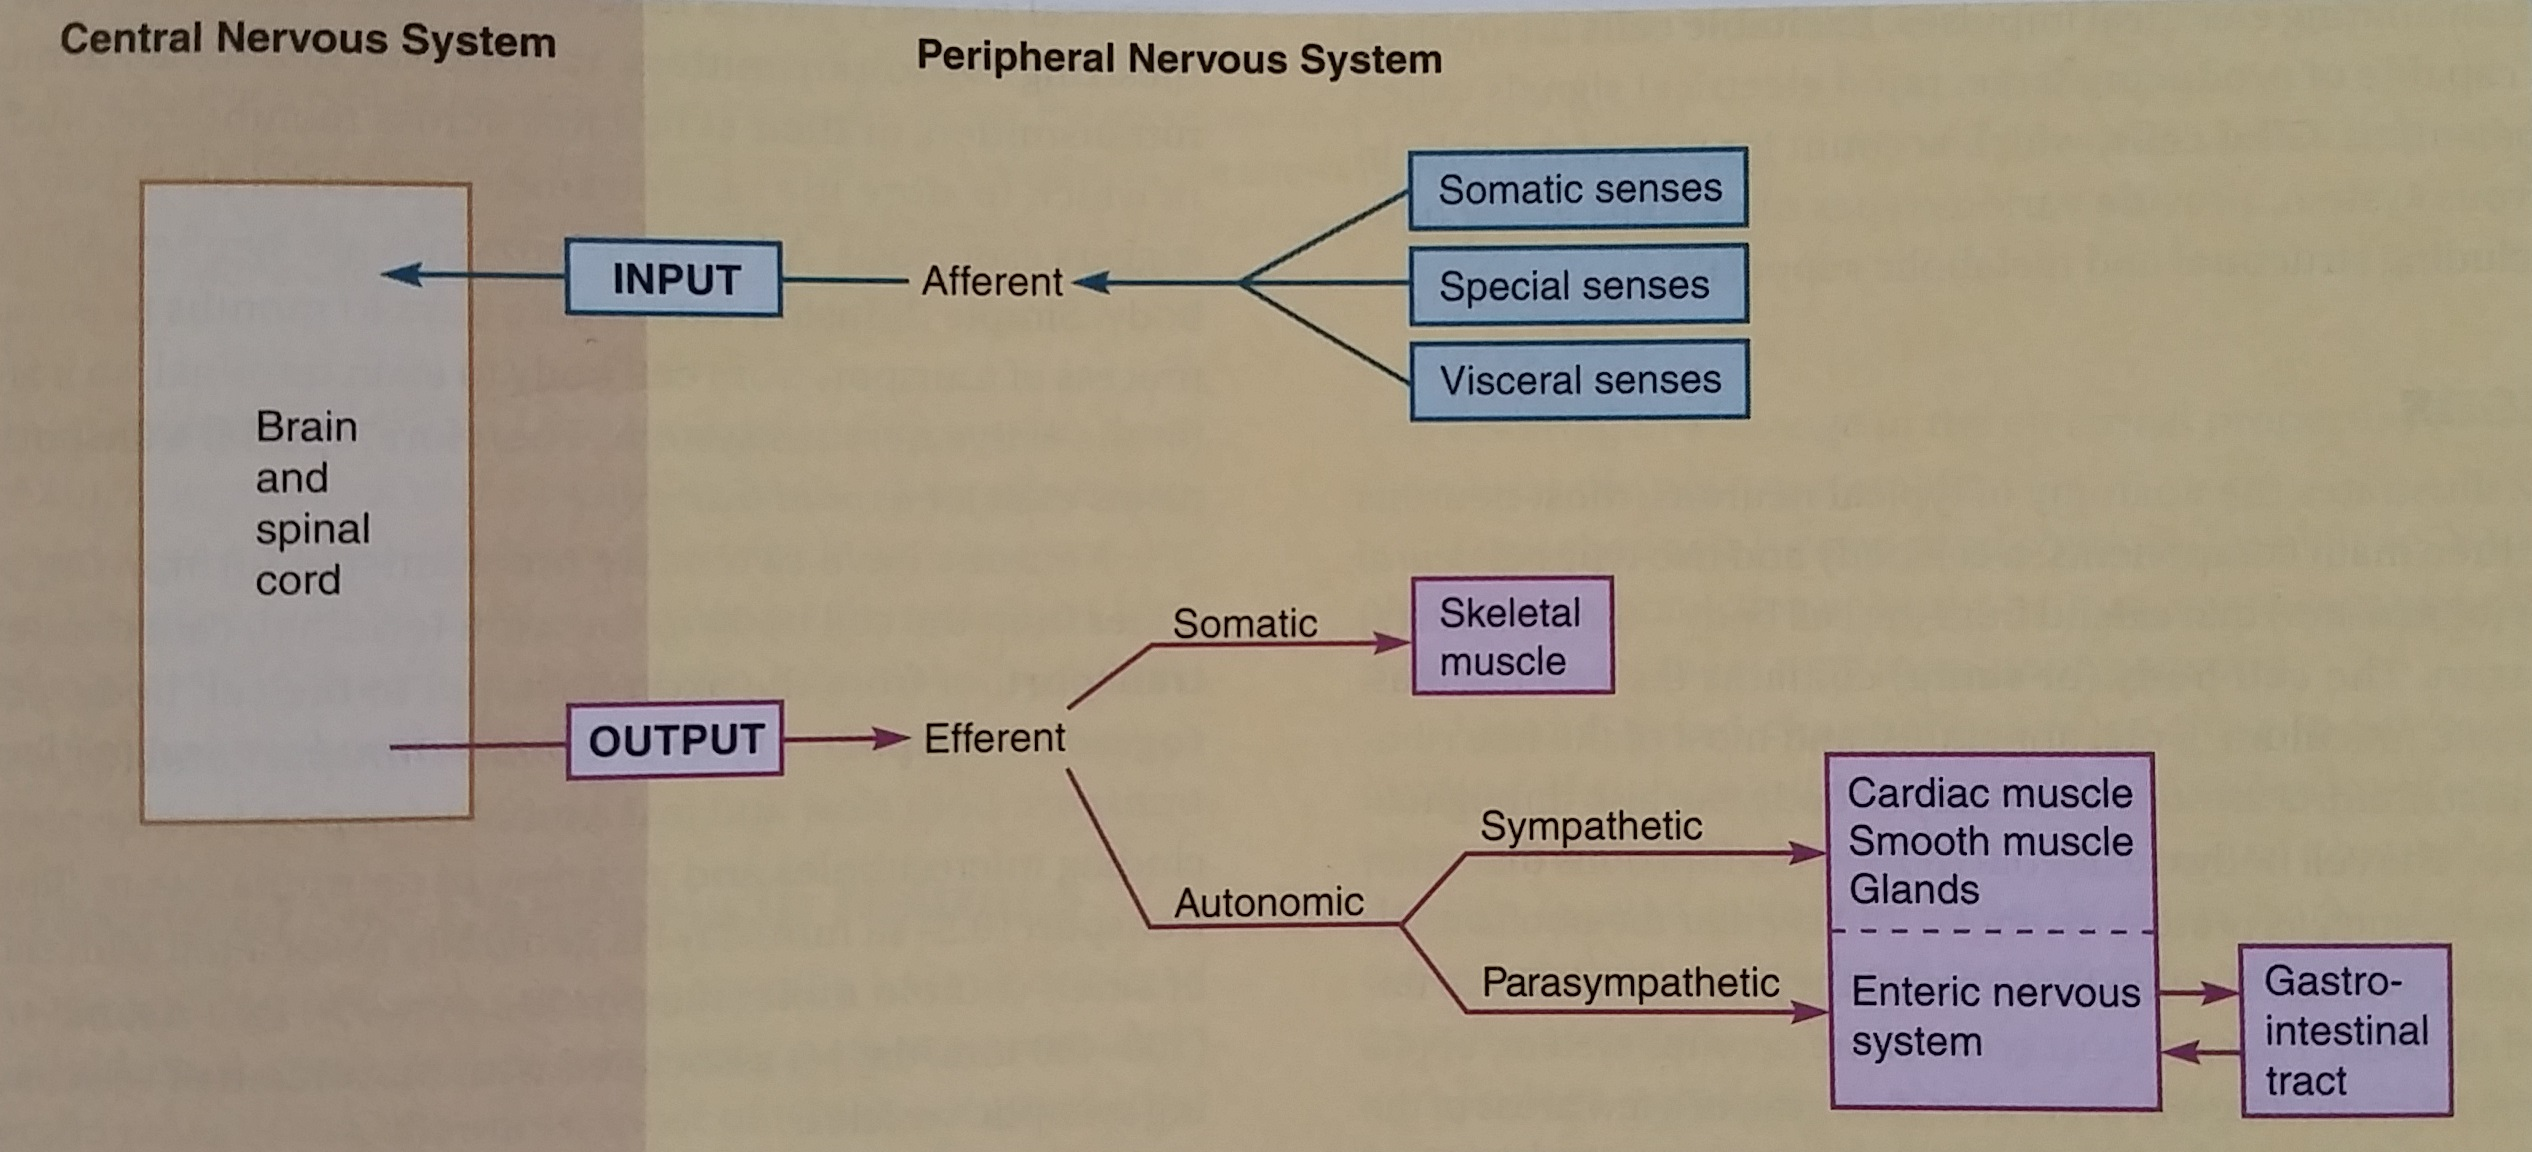
\includegraphics[scale=0.4]{figures/bProblemanalyse/Nervesys1.jpg}
	\caption{På figuren ses en opdeling af PNS og CNS samt hvordan et signal proceseres til en handling af nervesystemerne. \cite{Stanfield2014}}
	\label{Nersys}
\end{figure}

\section{Hjernens anatomi}
Cerebrum er encephalons største del og er involveret i sanseintegration, styring af frivillige bevægelser og højere intellektuelle funktioner, såsom tale og abstrakt tænkning. \cite{Academic2015b} Cerebrums ydre lag hedder cerebral cortex men kaldes hjernens grå substans. Her ligger nervers soma med dendritter. Cerebral cortex har forskellige centre, men kan også inddeles i højre og venstre halvdel. Delen af cerebral cortex der kontrollerer kroppens motorik med motor cortex kaldes gyrus præcentralis. Nerverne i dette område leder motoriske impulser til kroppens muskler igennem nervebanerne i den hvide substans, som indeholder nervernes axoner og fungerer derved som transportvej. \cite{Academic2015b,Martini2012,Stanfield2014} Disse axoner krydses i medulla oblongata og medulla spinalis og løber derefter til det modsatte legemeshalvdel fra, hvor impulsen afsendes. \cite{Martini2012}

Når en bevægelse udføres, starter det med en idé eller en intension om at lave en bevægelse. Denne tanke opstår i præfrontale cortex, som findes i lobus frontalis. Præfrontal cortex er specielt aktivt under udførelse af nye situationer / bevægelser og har forbindelse til motor cortex, som sætter indlærte bevægelser i gang. Samtidig modtager basalganglier i cerebellum signalet, hvorved kroppen kan modificere bevægelsen i forhold til omgivelserne. Cerebellum samarbejder altså med motor cortex, så bevægelsesplanen kan samles og sendes via de decenderende baner i rygmarven til bestemmelsesstedet. \cite{Bojsen-Moeller2012} \\
Hvis en bevægelse gentages, vil præmotor cortex gemme stimulationsmønstret. Dette gør, at bevægelsen kan udføres nemmere og mere præcist end ellers. Bevægelsen lagres i basalganglierne ved at synapseforbindelserne er styrket. \cite{Martini2012}

\section{Nervens anatomi}
En nerve består af soma, dendritter og et myelineseret akson. Soma indeholder cellekernen, endoplasmatisk reticulum, golgi apperater og de feste frie ribosomer. Indholdet i soma bestemmer, hvordan cellen agerer med andre samt dets funktion og vedligeholdelse. Dendritter er udløbere fra soma, som modtager impulser fra en anden nerve, og fører signalet ind til cellekroppen. Aksonet leder impulser fra soma til sin ende, der har mange små forgreninger kaldet aksonterminaler. Disse danner synapser med andre nervers dendritter eller targetorgan. \cite{Stanfield2014} \\
En nerve kan kun lede signaler, hvis der forekommer en høj nok elektrisk spændingsforskel mellem det intracellulær- og ekstracellulærvæske af membranen. Dette danner et aktionspotentiale. I en hvilende nerve er der et overskud af negative ioner i den intracellulære væske i forhold til i den ekstracellulære væske. Denne spændingsforskel mellem det intracellulæreog ekstracellulære kaldes membranpotentialet. \cite{Martini2012,Stanfield2014}

\section{Et biologisk signal}
